\section{Drehstrom-Leistungstransformator 50 Hz}
Der Transformator soll für die Außenaufstellung ausgelegt werden und wird von 3 AC \SI[]{50}[]{\Hz}, \SI[]{110}[]{\kilo\volt} gespeist.
Der Transformator soll ölgefüllt und selbstkühlend sein.\\ 



\subsection{Allgemeine Merkmale}

\begin{table}[htb]
    \centering
    \begin{NiceTabular}{|l|c|}[]
        \CodeBefore
        \columncolor{lightergray}{1}
        \Body
        \hline
         Aufstellung & Freiluftaufstellung\\
         \hline
         Verschmutzung & Verschmutzungsgrad III (stark) \\
         \hline
         Aufstellungshöhe & < 1000 m üNN\\
         \hline
         Umgebungstemperatur &  -30°C bis 40°C\\
         \hline
         Klimabedingungen & Normal\\ 
         \hline
                 \Block{3-1}{Dokumentationen} &  \tabitem Technische Zeichnungen und CAD\\
                         &\tabitem Montageplan, Wartungsplan, Dokumentationen\\
                         &\tabitem Prüfprotokoll der zu erfüllenden Prüfungen\\
                         \hline
       
    \end{NiceTabular}
\end{table}

\pagebreak
\subsubsection*{Normen}

\begin{itemize}[noitemsep]
    \item DIN VDE 0532-76-1: Leistungstransformatoren\cite*{DINEN600761.}
    \item DIN EN 60076-3 Leistungstransformatoren Teil 3: Isolationspegel, Spannungsprüfungen und äußere Abstände in Luft \cite*{DINEN600763VDE0532763:201903.}
    \item DIN 60076-4 Leistungstransformatoren Teil 4: Leitfaden zur Blitz- und Schaltstoßspannungsprüfung von Leistungs-
    transformatoren und Drosselspulen\cite*{DINEN600764.2003}
    \item DIN 60076-10 Leistungstransformatoren Teil 10: Bestimmung der Geräuschpegel\cite*{DINEN600761.2002}
    \item DIN EN 60071-1 Isolationskoordination Teil 1: Begriffe, Grundsätze und Anforderungen\cite*{DINEN600711.2010}
\end{itemize} 

\subsubsection*{Schaltbild}
\begin{figure}[htb]
\centering
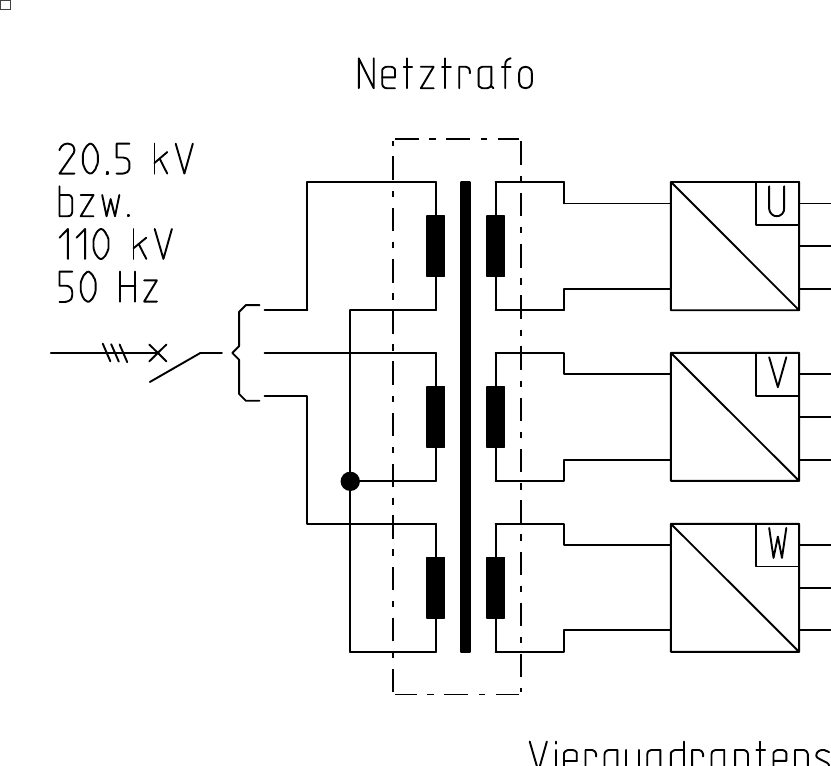
\includegraphics[width=\textwidth/2,frame]{Bilder/netztrafo.png}
\end{figure}
\subsection{Bemessungsdaten:}

\begin{table}[htb]
    \centering
    \begin{NiceTabular}{|l|p{2cm}|p{2cm}|}[hvlines]
        \CodeBefore
        \columncolor{lightergray}{1}
        \Body
       \Block{2-1}{Schaltgruppe} & OS & US \\ 
                                & Y(N) &   i0i0i0  \\
         Nennleistung ohne Leistung der Filterwicklung & \Block{1-2}{$\SI{17.68}{\unit{\mega\volt\ampere}}$}\\
         Nennspannung OS (Klemmenspannung) & \Block{1-2}{$\SI{110}{\kV}$}\\
         Max. Spannung OS (Klemmenspannung) & \Block{1-2}{$\SI{123}{\kV}$}\\
         Nennspannung US (Klemmenspannung) & \Block{1-2}{$\SI{3536}{\V}$}\\
         Nennstrom der US bei Nennspannung & \Block{1-2}{$\SI{1.667}{\kilo\ampere}$}\\
    \end{NiceTabular}
\end{table}

\textbf{Relative Kurzschlussspannungen:}
\begin{itemize}
    \item Bezugsgrößen: \\ bezogen auf Nennleistung bei $\SI{75}{\degree}$C; eine US Wicklung kurzgeschlossen; alle anderen Wicklungen offen; Speisung in OS Wicklung
    \item Werte \\ $uk_\mathrm{OS_iUS_i}\mathrm{(mit\,i=1...3)}=20\% (20.9\%...23.1\%)$; bezogen auf Nennleistung\\ $uk_\mathrm{US-US}>22\%$ (für alle Paarungen)
\end{itemize}

\subsubsection*{Verluste}
\begin{table}[htb]
    \centering
    \begin{NiceTabular}{|l|c|c|}[hvlines]
        \CodeBefore
        \columncolor{lightergray}{1}
        \Body
        &Grundschwingung&Umrichterbetrieb (Zusatzverluste)\\
        Leerlaufverluste bei Nennspannung &  tbd. kW&<1\% von der Grundschwingung\\
        Kurzschlußverluste bei 75 °C &tbd. kW&<1\% von der Grundschwingung\\
    \end{NiceTabular}
\end{table}
\clearpage

\subsubsection*{Stromwandler}

\begin{table}[!htb]
    \centering
    \begin{NiceTabular}{|l|c|}[hvlines]
        \CodeBefore
        \columncolor{lightergray}{1}
        \Body
        \Block{2-1}{Stromwandler OS-Seite} &  3xtbd/1A; 15VA; 10P10\\
                                & 3xtbd/1A; 15VA; 0,5 FS10\\
                                Stromwandler US-Seite &3x tbd/1A;15VA;10P10\\
                                Stromwandler Kesselschutz &1x 100/1A;3VA;5P20\\
    \end{NiceTabular}
\end{table}

\subsubsection*{Durchführungen}
\begin{table}[h]
    \centering
    \begin{NiceTabular}{|l|c|}[hvlines]
        \CodeBefore
        \columncolor{lightergray}{1}
        \Body
        OS& 3 (+1 optional Sternpunkt herausführbar)\\
        US & 3x2 \\
    \end{NiceTabular}
\end{table}

\textbf{Isolation (nach Prüfungsnorm in \cite*{DINEN600763VDE0532763:201903.}):}
\begin{table} [h]
    \centering
    \begin{NiceTabular}{|l|c|c|}[hvlines]
        \CodeBefore 
        \columncolor{lightergray}{1}
        \Body
             & OS & US gegen Erde \\ 
           max. Betriebsspannung  & $\SI{123}{\kilo\volt}$ &  $\SI{7.2}{\kilo\volt}$ \\
         Nennstehwechselspannung & $U_1=$\SI{185}{\kilo\volt}; $U_2=$\SI{230}{\kilo\volt}& \SI{20}{\kilo\volt} \\
         Nennstehblitzspannung & $U_1=$\SI{450}{\kilo\volt}; $U_2=$\SI{550}{\kilo\volt}&$U_1=$\SI{40}{\kilo\volt}; $U_2=$\SI{60}{\kilo\volt}\\
    \end{NiceTabular}
\end{table}

\subsubsection*{Sternpunktausführung}
Der Sternpunkt OS ist aus der Wicklung herauszuführen und eine spätere Verwendung vorzubereiten. Durchführung und Isolator sind nicht erforderlich, der Sternpunkt kann blind verflanscht werden. 

\textbf{Kapazitive Kopplung}\\
Eine kapazitive Übertragung von Blitzüberspannungen von der OS-Wicklung auf die US-Wicklung ist zu vermeiden. Bisherige Transformatoren in Bahnkupplungen hatten zu diesem Zweck Schirmwicklungen. 
 
\textbf{Geräuschpegel}\\
Aufstellungsort: Allgemeines Wohngebiet gemäß § 1 BImSchG  $L_\mathrm{pmax}=40 dB(A)$.
Grenzwert darf im Fernfeld(5m) mit Messung nach DIN EN 60076-10 nicht überschritten werden.
